Neste experimento busca-se utilizar aprendizado não supervisionado com o classificador \textit{k-means} de modo a obter o melhor valor de \textit{k}. Além disto busca-se reduzir a dimensão do conjunto de dados de modo a reter 90\% de variância.

\subsection{Descritor LBP}
\subsubsection{Redução de dimensionalidade}

Buscou-se reduzir a dimensionalidade do conjunto de dados obtidos com o descritor LBP de modo a reter 90\% de variância. Primeiramente os dados foram normalizados com a técnica Standard, ou seja, são calculados a média e o desvio padrão da conjunto de amostras, em seguida é subraída de cada amostra a média, o resultado então é divido pelo desvio padrão. Esta técnica foi selecionada pois obteve resultado levemente superior as outras técnicas na Seção~\ref{pratica02}.

Com a técnica PCA para redução de dimensionalidade foi selecionado o menor número de componentes que retinha 90\% de variância. Ver Figura~\ref{fig:points_pca_lbp}. Foi possível reduzir de 256 para 133 característica.

\begin{figure}[!htbp]
	\centering
	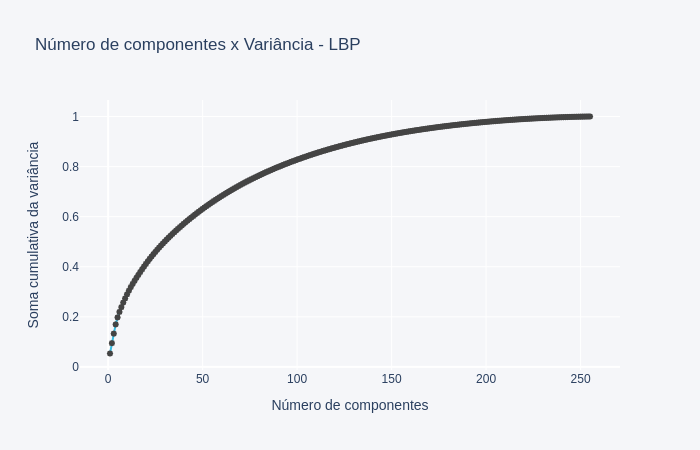
\includegraphics[width=1.0\linewidth,clip=true,trim=0cm 0cm 0cm 0cm, keepaspectratio=true]{points_pca_lbp.png}
	\caption{Selecionar o menor número de componentes retendo 90\% de variância.}
	\label{fig:points_pca_lbp}
\end{figure}

\subsubsection{Agrupamento}
Com a redução de dimensionalidade obtida foi utilizado o classificador k-means agrupando as amostras de 2 a 30 agrupamentos de forma iterativa. Ao fim, foi compilado e plotado a variância para cada quantidade de agrupamentos para aplicar o método elbow com intuito de definir a melhor quantidade de agrupamentos. O ponto mais distante da reta formada pela ligação do ponto inicial ao final foi 9, o melhor número de agrupamentos. Ver Figura~\ref{fig:points_elbow_lbp}. O agrupamento final foi plotado destancando-se os centróides na Figura~\ref{fig:scatter_k9_lbp}.

\begin{figure}[!htbp]
	\centering
	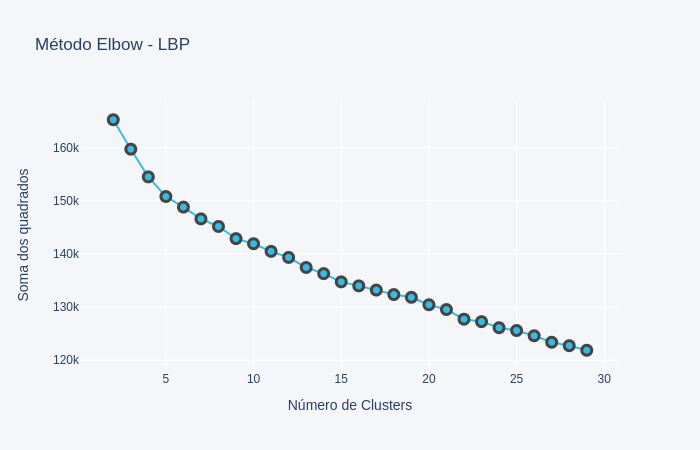
\includegraphics[width=1.0\linewidth,clip=true,trim=0cm 0cm 0cm 0cm, keepaspectratio=true]{points_elbow_lbp.png}
	\caption{Selecionar o melhor número de agrupamentos.}
	\label{fig:points_elbow_lbp}
\end{figure}

\begin{figure}[!htbp]
	\centering
	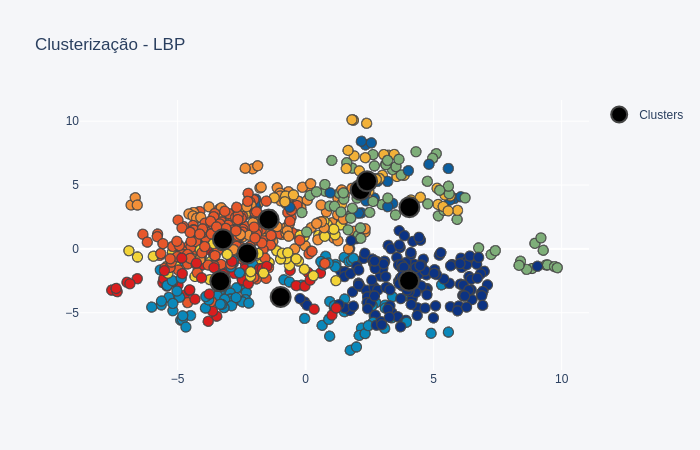
\includegraphics[width=1.0\linewidth,clip=true,trim=0cm 0cm 0cm 0cm, keepaspectratio=true]{scatter_k9_lbp.png}
	\caption{Conjuto de amostras agrupados em 9.}
	\label{fig:scatter_k9_lbp}
\end{figure}

\subsection{Descritor Gabor}
\subsubsection{Redução de dimensionalidade}
Foi aplicada a técnica PCA para as características extraídas com o descritor Gabor. Primeiramente os dados  foram normalizados com a técnica MinMax, melhor resultado obtido no experimento anterior. Foi possível reduzir as características de 60 para duas retendo 100\% de variância. Ver  Figura~\ref{fig:points_pca_gabor}.

\begin{figure}[!htbp]
	\centering
	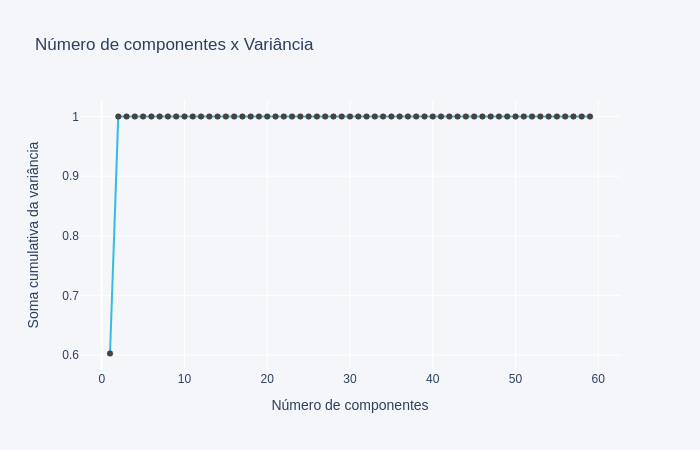
\includegraphics[width=1.0\linewidth,clip=true,trim=0cm 0cm 0cm 0cm, keepaspectratio=true]{points_pca_gabor.png}
	\caption{Selecionar o menor número de componentes retendo 100\% de variância.}
	\label{fig:points_pca_gabor}
\end{figure}

\subsubsection{Agrupamento}
Na sequência foi utilizado o classificador k-means agrupando as amostras de 2 a 30 agrupamentos de forma iterativa. Ao fim, foi compilado e plotado a variância para cada quantidade de agrupamentos para aplicar o método elbow com intuito de definir a melhor quantidade de agrupamentos. O ponto mais distante da reta formada pela ligação do ponto inicial ao final foi 8, o melhor número de agrupamentos. Ver Figura~\ref{fig:points_elbow_gabor}. O agrupamento final foi plotado destancando-se os centróides na Figura~\ref{fig:scatter_k8_gabor}.

\begin{figure}[!htbp]
	\centering
	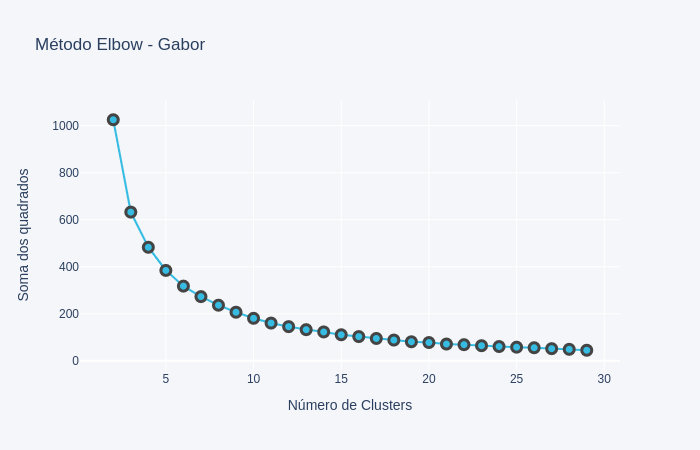
\includegraphics[width=1.0\linewidth,clip=true,trim=0cm 0cm 0cm 0cm, keepaspectratio=true]{points_elbow_gabor.png}
	\caption{Selecionar o melhor número de agrupamentos.}
	\label{fig:points_elbow_gabor}
\end{figure}

\begin{figure}[!htbp]
	\centering
	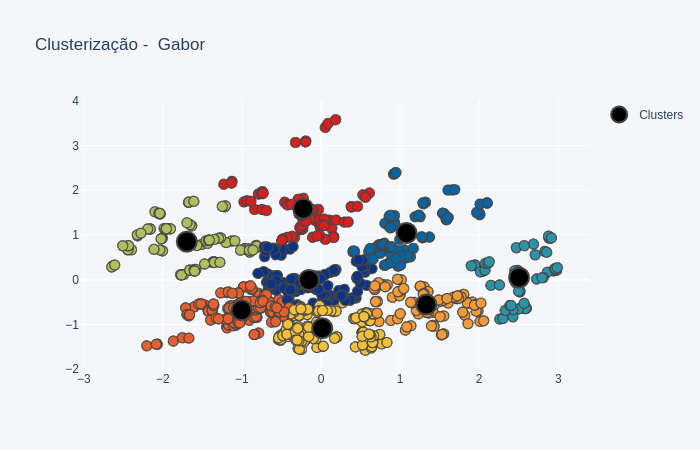
\includegraphics[width=1.0\linewidth,clip=true,trim=0cm 0cm 0cm 0cm, keepaspectratio=true]{scatter_k8_gabor.png}
	\caption{Conjuto de amostras agrupados em 8.}
	\label{fig:scatter_k8_gabor}
\end{figure}

Nota-se que o agrupamento plotado na Figura~\ref{fig:scatter_k8_gabor} possui fronteiras mais definidas do que na Figura~\ref{fig:scatter_k9_lbp}.

\subsubsection{Desenvolvimento} Prática 03 - ckplus - LBP - pca - kmeans; Prática 03 - ckplus - Gabor - pca - kmeans
\subsubsection{Exibição e Execução} ATUALIZAR
